\section[Общая схема протокола]{Общая идея}\label{sec:common_description}

\begin{enumerate}
  \item Алиса и Боб контролируют области пространства, необходимые для приготовления и измерения протяженных квантовых состояний.
  \item Расстояние $L$ между Алисой и Бобом всем известно и является параметром протокола. Алиса и Боб имеют часы, но не имеют общего начала отсчета времени (часы не синхронизированы).
  \item Алиса передает серию состояний. Отправка посылки происходит в один из двух моментов времени внутри интервала $\Delta T$, в какой именно~--- выбирается случайно (рис \ref{fig:timeline}). 
  Посылка представляет собой протяженное классическое состояние, состоящее из пары интенсивных когерентных пакетов, разделенных пространственно-временным интервалом $l_{pac}$, длина которого определяется исходя из свойств среды, в которой производится передача\footnote{Для передачи в воздухе пакеты должны быть разделены не менее, чем 1 метром пространства (см. приложение \ref{app:l_pac})}: 
  $|\alpha_c\rangle_1 \otimes|\alpha_c\rangle_2$ (индексы <<1>> и <<2>> отвечают пакетам, локализованным в моменты времени 1 и 2, рис \ref{fig:process}); среднее число фотонов в состоянии $\mu_c = |\alpha_c|^2 \gg 1$. 
  %Временное разрешение проводится с точностью до ширины пакета $l_{pac}$ (интервалы времени, меньшие $l_{pac} / c$, считаются нулевыми). 
  Момент времени $t_{A,i}$ посылки состояния в канал связи Алисой фиксируется по её часам.
  
  \begin{figure}[h]
  \center{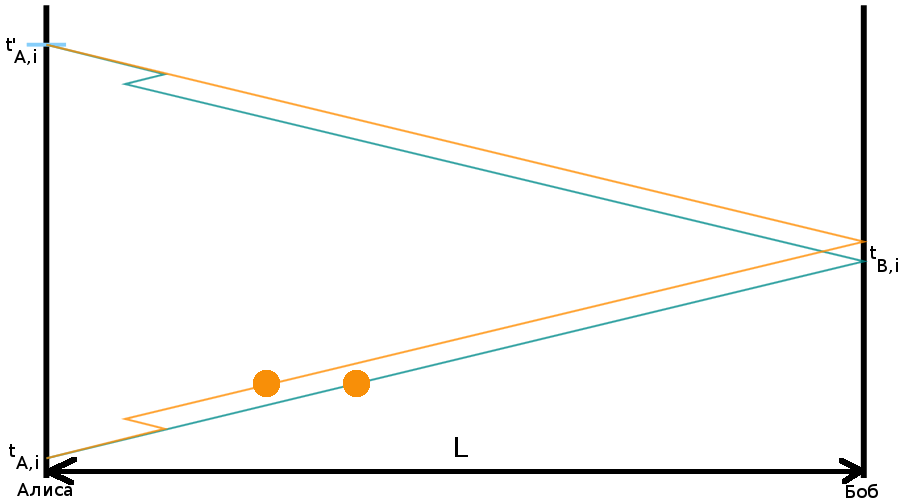
\includegraphics[width=0.9\linewidth]{not_catched}}
  \caption{Пространственно-временная диаграмма, поясняющая процесс приготовления, преобразования и распространения протяженных квантовых состояний.}
  \label{fig:process}
  \end{figure}
  \begin{figure}[h]
  \center{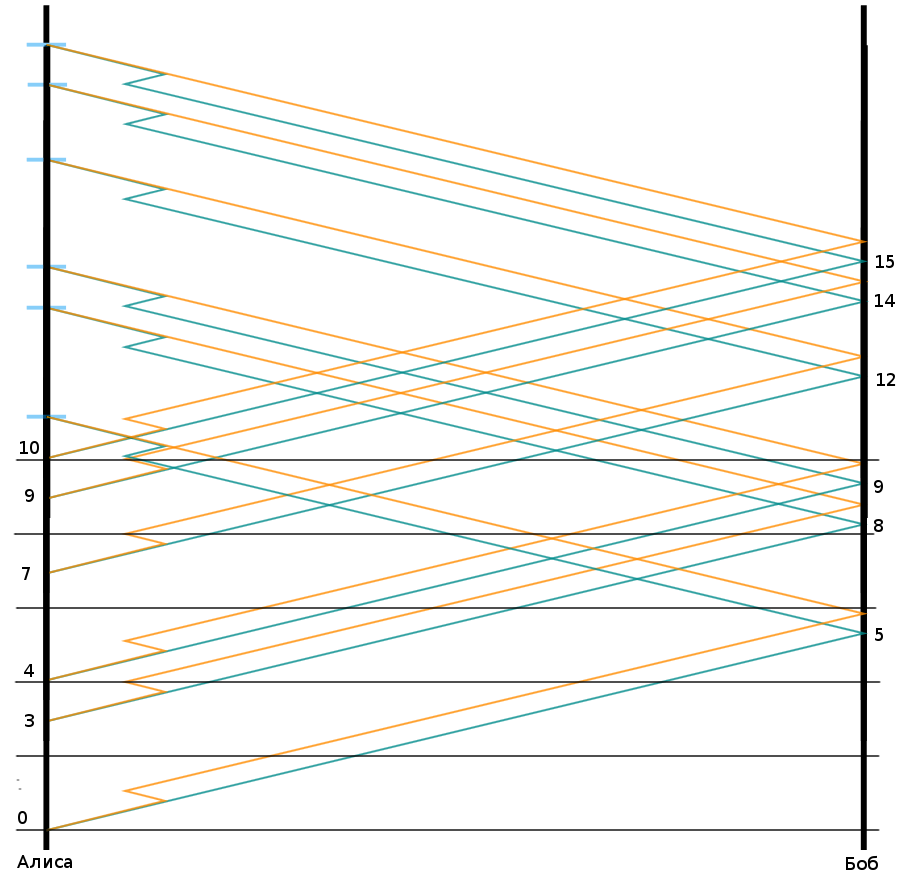
\includegraphics[width=0.9\linewidth]{timeline}}
  \caption{Пространственно-временная диаграмма, поясняющая посылку классических и прием квантовых состояний в случайные моменты. Слева и справа от вертикальный осей числами обозначены моменты посылки и приема состояний. }
  \label{fig:timeline}
  \end{figure}
  \begin{figure}[h]
  \center{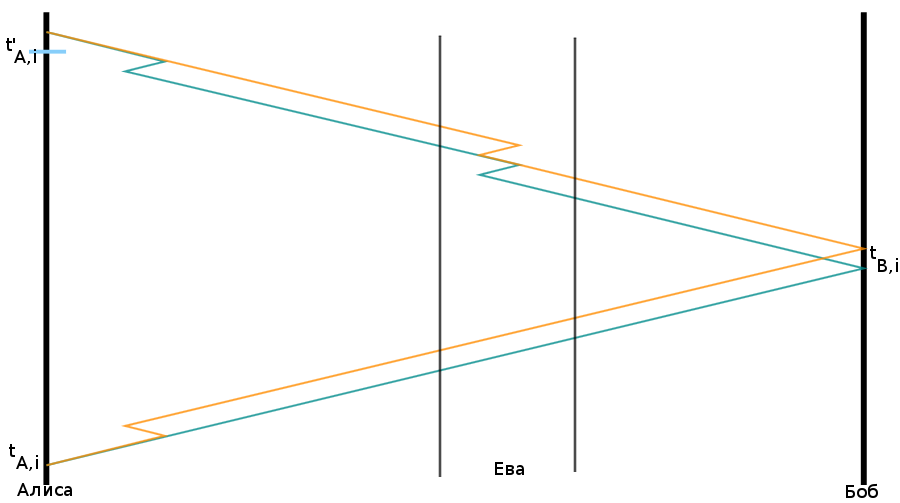
\includegraphics[width=0.9\linewidth]{eve_detected}}
  \caption{Пространственно-временная диаграмма, поясняющая причину задержек по времени протяженных состояний при подслушивании Евой}
  \label{fig:detected}
  \end{figure}
  
  \item На приемной стороне работает аппаратура Боба в ждущем режиме. Момент прихода $t_{B,i}$ каждой $i$-й посылки фиксируется быстрым классическим детектором. 
  Классический сигнал ослабляется до квазиоднофотонного уровня, на заднюю из <<половинок>> случайным образом навешивается фаза с помощью фазового модулятора. 
  Полученное состояние $|\alpha\rangle_1 \otimes |e^{i\varphi_B}\alpha\rangle_2$ ($\mu = |\alpha|^2 < 1$) возвращается обратно Алисе 
  \footnote{Все задержки на стороне Боба, связанные с обработкой, заранее известны. Их величина непринципиальна и считается включенной в моменты $t_{A,B,i}$ и $t'_{A,B,i}$.}. 
  Кодирование осуществляется на стороне Боба.
  Выбору логического 0 в ключе отвечает значение относительной фазы у двух импульсов $\varphi_B = \varphi_0$, а логической 1~--- $\varphi_B = \varphi_1$.   
  
  \item Алиса, зная расстояние $L$ и время отправки $t_{A,i}$ по своим часам своего состояния в канал связи, рассчитывает время прихода квантового состояния от Боба $t'_{A,i}$.
  В нужный момент включая фазовый модулятор, преобразует пришедшее состояние, случайным образом и независимо от Боба изменяя относительную фазу одной из <<половинок>>: 
  $|\alpha\rangle_1 \otimes |e^{i\varphi_B}\alpha\rangle_2 \rightarrow |\frac{\alpha}{2}\rangle_1 \otimes |\frac{(e^{i\varphi_B} - e^{i\varphi_A})\alpha}{2}\rangle_2$
  ($\varphi_A = \varphi_0$ или $\varphi_A = \varphi_1$), и производит измерения \textit{только в определенном временном окне}. 
  Если $\varphi_A \neq \varphi_B$, то возникает отсчет в детекторе, а если $\varphi_A = \varphi_B$, то отсчета не возникает в силу деструктивной интерференции. В результате отсчета Алиса достоверно знает, какой бит ключа посылал Боб.
  
  \item После проведения серии посылок стороны обмениваются интервалами времени между соседними посылками (рис \ref{fig:timeline}), которые каждый фиксировал по своим часам, и сравнивают их между собой. Подсчитывается доля их несовпадений $\eta$. Соседние посылки, интервалы между которыми не совпали, Алиса и Боб отбрасывают.
  
  \item Далее часть оставшейся последовательности раскрывается и сравнивается для оценки вероятности ошибки. Если ошибка меньше критической, происходит исправление ошибок через открытый классический канал связи и сжатие очищенного ключа. В результате возникает секретный ключ, известный только Алисе и Бобу.
\end{enumerate}

Нужно заметить, что Алиса и Боб не должны следить за средним числом долетевших посылок. Потери в канале связи не входят в критерий секретности ключей (\S\ref{sec:key_length}).
\clearpage
